% !TEX encoding = UTF-8 Unicode
% !TEX TS-program = xelatex
\chapter{多項式圖形}


\begin{tikzpicture}[line cap=round,line join=round,x=1.0cm,y=0.2cm]
\draw[-{Stealth[scale=1,angle'=45]},color=black] (-3.2,0.) -- (3.2,0)  node[] {$x$};
\draw[-{Stealth[scale=1,angle'=45]},color=black] (0,-19.2) -- (0,10)  node[above] {$y$};

\draw[line width=1.2pt,smooth,samples=100,domain=-2.35:3] plot(\x,{1*(\x +2.2 )*(\x -0.5) *(\x - 1.5)*(\x -2.7) }) ;
\node [above ] at (1,10){ $y = f(x)$};
%畫上
\foreach \v in 
{-3,-2,-1,1,2,3}
{
    \draw[shift={(\v,0)},color=black] (0pt,2pt) -- (0pt,-2pt) node[below] { $\v$};
};

%\draw[ultra thick,fill] (1.5,-2) circle (0.8pt) node [ below] {$(1.5,-2)$};

\end{tikzpicture}

    \begin{tikzpicture}[line cap=round,line join=round,x=1.0cm,y=0.1cm]
\draw[-{Stealth[scale=1,angle'=45]},color=black] (-2.1,0.) -- (3,0.)  node[] {$x$};

\draw[line width=1.2pt,smooth,samples=100,domain=-1.1:2.3] plot(\x,{-6.4*(\x +1)*(\x -1) *(\x - 2)*(\x -2) }) ;
\node [above ] at (1,10){ $y = f(x)$};
%畫上
\foreach \v in 
{-1,0,1,2}
{
    \draw[shift={(\v,0)},color=black] (0pt,2pt) -- (0pt,-2pt) node[above] { $\v$};
};

\draw[ultra thick,fill] (1.5,-2) circle (0.8pt) node [ below] {$(1.5,-2)$};

\end{tikzpicture}

\begin{tikzpicture}
\coordinate (cLineL) at (-4, 0);
\coordinate (cLineR) at (6, 0);
\coordinate (cAL) at (-3,0);
\coordinate (cAR) at (5,0);

\draw  (cLineL) -- (cLineR);
\draw[ultra thick]  (cAL) -- (cAR);

\begin{scope}[shift={(0,0.5)}]
\def\Bradius{4}
\coordinate (cBC) at (1, 0);
\coordinate (cBR) at (1 + \Bradius, 0);
\coordinate (cBL) at (1 - \Bradius, 0);
\draw [-{Stealth[scale=1.3,angle'=45]},semithick]  (cBC) -- (cBR);
\draw [-{Stealth[scale=1.3,angle'=45]},semithick]  (cBC) -- (cBL);
\draw[ultra thick,fill] (cBC) circle (0.8pt);
\end{scope}


\foreach \v in 
{   1
}
{
    \begin{scope}[shift={(0,0.5)}]
    \def\Bradius{4}
    \coordinate (cBC) at (\v, 0);
    \coordinate (cBR) at (\v + \Bradius, 0);
    \coordinate (cBL) at (\v - \Bradius, 0);
    \draw [-{Stealth[scale=1.3,angle'=45]},semithick]  (cBC) -- (cBR);
    \draw [-{Stealth[scale=1.3,angle'=45]},semithick]  (cBC) -- (cBL);
    \draw[ultra thick,fill] (cBC) circle (0.8pt);
    \end{scope}
};

\foreach \v/\u/\t in 
{   cAL/270/$-3$,
    cAR/270/$5$,
    cLineL/180/$B$
}
{
    \draw[ultra thick,fill] (\v) circle (0.8pt);
    \node[label=\u:\t] at (\v){};
};

\end{tikzpicture}

\begin{tikzpicture}[line cap=round,line join=round,x=2cm,y=1cm]
\draw[-{Stealth[scale=1,angle'=45]},color=black] (0.9,0.) -- (4.5,0.)  node[] {$x$};
%\draw[-{Stealth[scale=1,angle'=45]},color=black] (0.,-4.) -- (0.,1.5) node[above] {$y$};
\foreach \x in {1,2,3,4}
\draw[shift={(\x,0)},color=black] (0pt,2pt) -- (0pt,-2pt) node[below] {\footnotesize $\x$};
\draw[line width=1.2pt,smooth,samples=100,domain=1:4] plot(\x,{-1*((\x -1)*(\x-2)*(\x-3)*(\x-4))}) node [above ] { $y = f(x)$};
\node [ above ] at (1.5,0) {$R_1$};
\node [ below ] at (2.5,0) {$R_2$};
\node [ above ] at (3.5,0) {$R_3$};
\end{tikzpicture}

\begin{tikzpicture}[line cap=round,line join=round,x=2cm,y=1cm]
\draw[-{Stealth[scale=1,angle'=45]},color=black] (0.9,0.) -- (2.5,0.)  node[] {$x$};
\draw[-{Stealth[scale=1,angle'=45]},color=black] (0.,-4.) -- (0.,1.5) node[above] {$y$};
\foreach \x in {1,2,3,4}
\draw[shift={(\x,0)},color=black] (0pt,2pt) -- (0pt,-2pt) node[below] {\footnotesize $\x$};
\draw[line width=1.2pt,smooth,samples=100,domain=-0.1:2.1] plot(\x,{3*((\x )*(\x-2))}) node [above ] { $y = f(x)$};

\draw[ultra thick,fill] (1,0) circle (1pt) node [ above left] {$B(-1,0)$};
\draw[ultra thick,fill] (2,0) circle (1pt) node [ above ] {$A(0,0)$};
\draw[ultra thick,fill] (3,-3) circle (1pt) node [ below] {$C(1,-3)$};

\end{tikzpicture}

\begin{tikzpicture}[line cap=round,line join=round,x=0.5cm,y=0.5cm]
\draw[-{Stealth[scale=1,angle'=45]},color=black] (0,0.) -- (10,0.)  node[] {$x$};
%\foreach \x in {-3,-2,-1,1,2}
%\draw[shift={(\x,0)},color=black] (0pt,2pt) -- (0pt,-2pt) node[below] {\footnotesize $\x$};
\draw[-{Stealth[scale=1,angle'=45]},color=black] (0.,0) -- (0.,10) node[above] {$y$};
%\foreach \y in {1,2}
%\draw[shift={(0,\y)},color=black] (2pt,0pt) -- (-2pt,0pt) node[left] { $\y$};
\draw[line width=1.2pt,smooth,samples=100,domain=3:7] plot(\x,{0.33*((\x -5 )*(\x-5) * (\x-5))+\x}) node [above ] { $y = f(x)$};
%畫上
\foreach \v in 
{5}
{
    \draw[shift={(\v,0)},color=black] (0pt,2pt) -- (0pt,-2pt) node[below] { $\v$};
};
\end{tikzpicture}

\begin{tikzpicture}[line cap=round,line join=round,x=1.0cm,y=1cm]
\draw[-{Stealth[scale=1,angle'=45]},color=black] (-2.1,0.) -- (3,0.)  node[] {$x$};
%\foreach \x in {-3,-2,-1,1,2}
%\draw[shift={(\x,0)},color=black] (0pt,2pt) -- (0pt,-2pt) node[below] {\footnotesize $\x$};
\draw[-{Stealth[scale=1,angle'=45]},color=black] (0.,-1.) -- (0.,2.5) node[above] {$y$};
\foreach \y in {1,2}
\draw[shift={(0,\y)},color=black] (2pt,0pt) -- (-2pt,0pt) node[left] { $\y$};

%\draw[color=black] (0pt,-10pt) node[] {\footnotesize $0$};
%\clip(-3.1,-15.) rectangle (2.3,35.);
\draw[line width=1.2pt,smooth,samples=100,domain=-1.3:3] plot(\x,{0.3*((\x -2 )*(\x-2) * (\x+1))}) node [above ] { $y = f(x)$};
%畫上
\foreach \v in 
{1}
{
    \draw[shift={(\v,0)},color=black] (0pt,2pt) -- (0pt,-2pt) node[below] { $\v$};
};


\draw[ultra thick,fill] (-1,0) circle (0.8pt) node [ above left] {$B(-1,0)$};
\draw[ultra thick,fill] (2,0) circle (0.8pt) node [ below] {$A(2,0)$};

\end{tikzpicture}

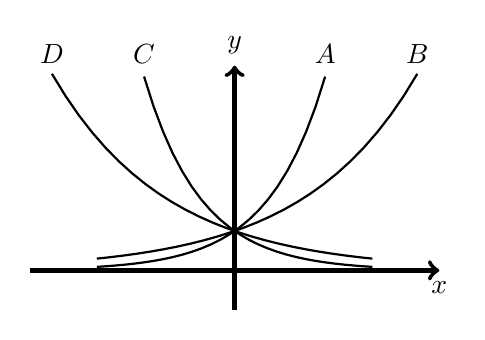
\begin{tikzpicture}[scale=.5]
\draw[ultra thick, ->] (-5.2,0) -- (5.2,0) node[below] {$x$};
\draw[ultra thick, ->] (0,-1) -- (0,5.2) node[above] {$y$};
%        \draw[very thin,color=gray] (-5,-1) grid (5,5);
\draw[thick, color=black, domain=-3.5:4.64] plot (\x,{2^(\x/2)});
\draw[thick, color=black, domain=-3.5:2.3] plot (\x,{2^(\x)});
\draw[thick, color=black, domain=-4.64:3.5] plot (\x,{2^(-\x/2)});
\draw[thick, color=black, domain=-2.3:3.5] plot (\x,{2^(-\x)});
\node[above] at (4.64, 5) {$B$};
\node[above] at (2.3, 5) {$A$};
\node[above] at (-4.64, 5) {$D$};
\node[above] at (-2.3, 5) {$C$};

\end{tikzpicture}

\begin{tikzpicture}[line cap=round,line join=round,x=1.0cm,y=0.1cm]
\draw[-{Stealth[scale=1,angle'=45]},color=black] (-3.1,0.) -- (2.6,0.);
%\foreach \x in {-3,-2,-1,1,2}
%\draw[shift={(\x,0)},color=black] (0pt,2pt) -- (0pt,-2pt) node[below] {\footnotesize $\x$};
%\draw[->,color=black] (0.,-15.) -- (0.,35.);
%\foreach \y in {-10,10,20,30}
%\draw[shift={(0,\y)},color=black] (2pt,0pt) -- (-2pt,0pt) node[left] {};

%\draw[color=black] (0pt,-10pt) node[] {\footnotesize $0$};
%\clip(-3.1,-15.) rectangle (2.3,35.);
\draw[line width=1.2pt,smooth,samples=100,domain=-3.1:2.3] plot(\x,{0.01*(2.0*(\x)-1.0)^(3.0)*((\x)^(2.0)-4.0)^(3.0)*((\x)+3.0)^(2.0)});


\foreach \v in 
{   -3,-2,2,-3
}
{
    \draw[ultra thick,fill] (\v,0) circle (0.8pt);
    \node[above] at (\v,0){$\v$};
};

\draw[ultra thick,fill] (0.5,0) circle (0.8pt);
\node[above] at (0.5,0){$\frac{1}{2}$};
\end{tikzpicture}
\def\FunctionG(#1){+((#1) + 0.5)*((#1) -2)* ((#1) -4)}%
\begin{tikzpicture}
\begin{axis}[
%axis y line=center,
%axis x line=middle, 
%axis on top=true,
xmin=-2,
xmax=6,
ymin=-5,
ymax=24,
height=6.0cm,
width=8.0cm,
%grid,
%xtick={-1,...,5},
%ytick={-40,-32,...,40},
hide y axis,
hide x axis,
]
\addplot [domain=-1.5:5, samples=50, mark=none, ultra thick] {\FunctionG(x)};
\draw[line width=1.7pt,-{Stealth[scale=1,angle'=45]}] (axis cs:-2,0 ) -- (axis cs:5.5,0) node [] {$x$};
\draw[line width=1.7pt,-{Stealth[scale=1,angle'=45]}] (axis cs:0,-5 ) -- (axis cs:0,20) node [left] {$y$};
\node [left] at (axis cs: 3.6,10) {$y=f(x)$};

\end{axis}
\end{tikzpicture}
\def\FunctionF(#1){+((#1) + 0.5)*((#1) -2)* ((#1) -4)}%
\begin{tikzpicture}
\begin{axis}[
%axis y line=center,
%axis x line=middle, 
%axis on top=true,
xmin=-2,
xmax=6,
ymin=-5,
ymax=24,
height=6.0cm,
width=8.0cm,
%grid,
%xtick={-1,...,5},
%ytick={-40,-32,...,40},
hide y axis,
hide x axis,
]
\addplot [domain=-1.5:5, samples=50, mark=none, ultra thick] {\FunctionF(x)};
\draw[line width=1.7pt,-{Stealth[scale=1,angle'=45]}] (axis cs:-2,0 ) -- (axis cs:5.5,0) node [] {$x$};
\draw[line width=1.7pt,-{Stealth[scale=1,angle'=45]}] (axis cs:0,-5 ) -- (axis cs:0,20) node [left] {$y$};
\node [left] at (axis cs: 3.6,10) {$y=f(x)$};
%\draw[ultra thick] (axis cs:-1,0) circle (2pt);
%\draw[ultra thick] (axis cs: 2,0) circle (2pt);
%\draw[ultra thick] (axis cs: 4,0) circle (2pt);
%\node [below] at (axis cs: -1,0) {$-1$};
%\node [below] at (axis cs: 2,0) {$2$};
%\node [below] at (axis cs: 4,0) {$4$};
\end{axis}
\end{tikzpicture}

\section{勘根}
    \begin{tikzpicture}[scale=1]
\draw[-{Stealth[scale=1.3,angle'=45]},semithick] (0,0) -- (8.5,0) node[] {$x$};
\foreach \v in 
{1,2,3,4,5,6,7}
{
    \draw[ultra thick,fill] (\v,0) circle (1pt);
    \node[label={270:$\v ^2$}] at (\v,0){};
};
\foreach \v/\u in 
{0/1,2/3,4/5,6/7}
{
    \draw [semithick] (\v,0) -- (\u,0) node [midway, below] {$-$};
};
\foreach \v/\u in 
{1/2,3/4,5/6,7/8}
{
    \draw [semithick] (\v,0) -- (\u,0) node [midway, above] {$+$};
};

\end{tikzpicture}

    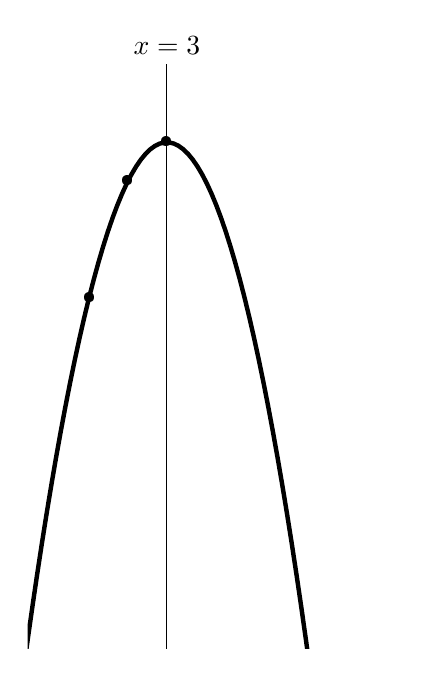
\begin{tikzpicture}
\makeatletter
\tikzset{
    nomorepostaction/.code=\makeatletter\let\tikz@postactions\pgfutil@empty, % From http://tex.stackexchange.com/questions/3184/applying-a-postaction-to-every-path-in-tikz/5354#5354
    my axis/.style={
        postaction={
            decoration={
                markings,
                mark=at position 1 with {
                    \arrow[ultra thick]{latex}
                }
            },
            decorate,
            nomorepostaction
        },
        thin,
        -, % switch off other arrow tips
        every path/.append style=my axis % this is necessary so it works both with "axis lines=left" and "axis lines=middle"
    }
}
\makeatother
\pgfplotsset{ticks=none}
\begin{axis}[
unit vector ratio*=1 1 1,
axis lines = middle,
axis line style = {my axis},
hide y axis,
hide x axis,
width=11cm,
xlabel={$x$},
ylabel={$y$},
ymax =12,
ymin =-4,
xmax = 10,
xmin = 
]
%Below the red parabola is defined
\addplot [
domain=-3:9, 
samples=100, 
color=black,ultra thick
]
{-x*x+6*x};
%\addlegendentry{$\$}
%Here the blue parabloa is defined
\draw (axis cs:3,-10) -- (axis cs:3,11) node [above] {$x=3$};
\node at (axis cs:1, 5) {\textbullet};
\node at (axis cs:2, 8) {\textbullet};
\node at (axis cs:3, 9) {\textbullet};
%    \foreach \Point in {(axis cs:1, 5), (axis cs:2,8), (axis cs:3,9)}{
%    \node at \Point {\textbullet};
%};

\end{axis}
\end{tikzpicture}

\pgfmathdeclarefunction{myfunct}{1}{%
    \pgfmathparse{-1*(#1+0.5)*(#1-1.5)}%
}
\begin{tikzpicture}
%\pgfplotsset{ticks=none}
\begin{axis}[
unit vector ratio*=1 1 1,
axis lines = middle,
axis line style = {-{Stealth[scale=1.3,angle'=45]}},
%hide y axis,
%hide x axis,
width=7cm,
xlabel={$x$},
ylabel={$y$},
xtick={-2,-1,...,3},
ymax =2.5,
ymin =-4.5,
xmax = 3.5,
xmin = -2.5
]
%Below the red parabola is defined
\addplot[samples=100,domain=-2:3] {myfunct(x)};
%\addlegendentry{$\$}
%Here the blue parabloa is defined



\end{axis}
\end{tikzpicture}

    \pgfmathdeclarefunction{myfunct2}{1}{%
    \pgfmathparse{-1*(#1-3)^2+2}%
}
\begin{tikzpicture}
%\pgfplotsset{ticks=none}
\begin{axis}[
unit vector ratio*=1 1 1,
axis lines = middle,
axis line style = {-{Stealth[scale=1.3,angle'=45]}},
hide y axis,
hide x axis,
width=7cm,
xlabel={$x$},
ylabel={$y$},
xtick={-2,-1,...,3},
ymax =2.5,
ymin =-4.5,
xmax = 8,
xmin = -2
]
%Below the red parabola is defined
\addplot[samples=100,domain=-2:8] {myfunct2(x)};
%\addlegendentry{$\$}
%Here the blue parabloa is defined
\pgfplotsinvokeforeach{1,2,3,4,5}{ 
    %    \addplot coordinates { (#1,0) (#1,{myfunct2(#1)}) }; \node[above=5pt] at (axis cs:#1,{myfunct2(#1)}) {\pgfmathprint{myfunct2(#1)}}; }
    
    \node at (axis cs:#1, {myfunct2(#1)}) {\textbullet };
    \node at (axis cs:#1, {myfunct2(#1)}) { $(#1, f(#1))$};
}

\end{axis}
\end{tikzpicture}